%\documentclass[11pt]{memoir}
\documentclass[10pt,english,a4paper,twoside,openright]{memoir}
% Packages
\usepackage[english]{babel}
\usepackage[draft,nomargin,inline,silent]{fixme}
\usepackage[font=footnotesize,format=plain,labelfont=bf,up]{caption}
\usepackage{lmodern}
\usepackage{pifont}
\usepackage{memhfixc}
\usepackage[T1]{fontenc}
\usepackage{multicol}
\usepackage[pdftex,
            colorlinks=false,
            pdfduplex=DuplexFlipLongEdge,
            pdfborder={0 0 0},
            pdftitle={s601a},
            pdfauthor={Jesper kjeldgaard},
            pdfsubject={},
            pdfkeywords={},
            plainpages=false
            ]{hyperref}
\usepackage[pdftex]{graphicx}  %enables images & angling of them
\usepackage{booktabs,multirow} %enables multirows in tables
\usepackage{supertabular} % enables super tables :=)
\usepackage{rotating} % landscape table
\pdfminorversion=5
%\RequirePackage{lineno} % enabling linenumbers

 % pseudocode
\usepackage{algorithmic}
\usepackage{subfig}
\usepackage{bbding}

\setlrmarginsandblock{3.5cm}{*}{0.5} % Right and left
\setulmarginsandblock{2.5cm}{*}{1.1}    % Top and bottom

% Change normal headers and footers
\makeoddhead{headings}{}{}{\small\rightmark}
\makeevenhead{headings}{\small\leftmark}{}{}

\makeoddfoot{headings}{}{}{\small\thepage}
\makeevenfoot{headings}{\small\thepage}{}{}

\makeheadrule{headings}{\textwidth}{\normalrulethickness}
\makefootrule{headings}{\textwidth}{\normalrulethickness}{\footruleskip}
%Instillinger til code farvning i lstlisting
\usepackage{listings}
\usepackage{color}
\usepackage[svgnames,tables,hyperref]{xcolor}
\lstset{language=Ruby,captionpos=b,tabsize=2,numbers=left,numberstyle=\tiny,numbersep=4pt,frameround=tttf,breaklines=true,frame=single,showstringspaces=false,
basicstyle=\color{black}\ttfamily\footnotesize,
stringstyle=\color{gray},
commentstyle=\color{gray}\itshape\ttfamily,
keywordstyle=\color{black}\bfseries\ttfamily}

% whitespace imellem paragraphs.
\setlength{\parskip}{0.20cm}
\setlength{\parindent}{0pt}

% make hyperlinks \href{}
\usepackage{hyperref}
\hypersetup{pdftex, colorlinks=true, linkcolor=blue, citecolor=blue, filecolor=blue, urlcolor=blue, pdftitle=, pdfauthor=jesper kjeldgaard, pdfsubject=, pdfkeywords=}

% used for citation
\usepackage{cite}

% for including graphics
\DeclareGraphicsExtensions{.png,.eps}

% for tables etc.
\usepackage{color}
\usepackage{array}

\usepackage{fancyhdr}
\pagestyle{fancy}


\begin{document}

% Title page
\meta{Includes Module code, Title, student name and number, and supervisor's
name.}

\thispagestyle{empty}
\cleardoublepage

% Use roman numbers on the start of the report
\pagenumbering{Roman}
% Use plain style
\thispagestyle{plain}

% \meta{A small summary of the whole project from start to finish.} 1/2 - 3/4
% page.
\begin{abstract}
In this project, a concurrent webserver is implemented in Ruby using the
Behaviour-Driven Development (BDD) method. 

Topics relevant to the thesis, namely webservers, concurrent programming, the
Ruby programming language and BDD are covered. The implementation of each
requirement is described, along with selected technical problems and their
solutions.

Yarn, the name of the produced webserver, is benchmarked to other Ruby
webservers and the results revealed that for static requests it performed
sub par other webservers, but for CPU intensive applications it performed quite
well.

Using BDD enabled getting started on the implementation right away, without
having to produce a big design upfront. This proved to be both a advantage and
a disadvantage, as some design decisions which turned out not to work as
expected, might have been avoided. As BDD employs a test-first approach, a
large test-suite was produced and having many tests enabled for design changes
late in the development, without having to worry about the correctness of the
implementation.
\end{abstract}


\cleardoublepage

% Create table of contents
\setcounter{secnumdepth}{2} % set numbering depth of sections and chapters
\setcounter{tocdepth}{2} % set numbering depth of table of contents
\addcontentsline{toc}{chapter}{Table of Contents}
\tableofcontents*

% Use temporary line numbers on all pages
% \setpagewiselinenumbers
% \modulolinenumbers[5]
% \linenumbers

% Main Contents of report, add chapters here
\chapter{Introduction}
\pagenumbering{arabic}
% \meta{A brief introduction to the project, with a clear definition 
% of the problem to be addressed, and guide to rest of the report.}
%
% What the thesis will say
Develop a Ruby webserver which takes advantage of multiple cores/processors.

\section{Readers Guide}
Background information required for the remainder of the report is covered in
Chapter~\ref{bg}. Chapter~\ref{an} covers the requirements for the software
developed. Chapter~\ref{im} regards implementation specific aspects of the
software and Chapter~\ref{te} describes the testing done during the
development. In Chapter~\ref{de}, the end product is demonstrated,
evaluated through a series of benchmarks and compared to other Ruby
webservers. In Chapter~\ref{re} the project process is reflected upon, and
Chapter~\ref{co} concludes the project and suggests future improvements to the
software.

For source code listings, the caption will show which file and on what line
the code is taken from. The source code is included on a CD, and also
available at \url{https://github.com/thejspr/yarn}.


\section{Acknowledgements}
I would like to thank Kai Xu for invaluable suporvision and feedback
throughout this project.


\chapter{Background}
\label{bg}
% \meta{This should describe the context of the project and should attempt to 
% establish the state of the art in the project area. This should show 
% evidence of scholarly activity in demonstrating the ability to research,
% collate and integrate information into a coherent document that uses 
% referencing and quotations correctly so that the background to the project
% can be quickly understood.}

\fixme{Bg intro}

\section{Development Method} % (fold)
\label{sec:development}
%intro
Software development methods are often used to manage the scope and complexity
of software projects. Some methods follow a linear approach and dictates first
the system is designed, then implemented and finally tested. Whilst this
approach works in many situations, it is critized for it's inability to handle
difficulties arising in the process. Another type of methods grouped as agile,
provides an interative process where the software is designed,
developed and tested through a series of iterations \cite{bddintro}. 
Two agile methods were considered for this project;
Behaviour-Driven Development (BDD) and Test-Driven Development (TDD).

BDD is an evolution of TDD which focus more on the
behaviour of the software instead of the software structure. A problem with
TDD is that it focus on the internals of the implementation structure, making
tests fail even when the behaviour of the code hasn't changed. In short TDD
tests what an object \textit{is} and BDD tests what an object
\textit{does}\cite{rspecbook}. Hence, BDD ensures business value is created and
the software works as intended, TDD ensures that the code is correct but is blind to
whether it provides the intended business value.

BDD was chosen as the development method for this project due to it being seen
as an improvement on TDD and allowing for rapid development without needing to
design the system up front. This agility makes it easier to handle
difficulties and caveats during the process, leaving more room to adapt. With
BDD (and TDD) the design is constantly evolving as more code is added and
former code is constantly reviewed and refactored. This form of design is
referred to as an emergent design. The following describes the BDD development
cycle and the tools used \cite{bddintro}.

\subsection{Behaviour-Driven Development}
%intro
BDD revolves around writing specifications for
what a program is intended to do. This process is made up of an outer and an
inner loop. The outer loop concerns passing an acceptance test covering one
feature i.e.\ logging functionality. The inner loop concerns passing RSpec
behaviour specifications describing the behaviour of methods and objects.
Figure~\ref{bdd_cycle} depicts the BDD cycle.

\begin{figure}[htb]
  \centering
  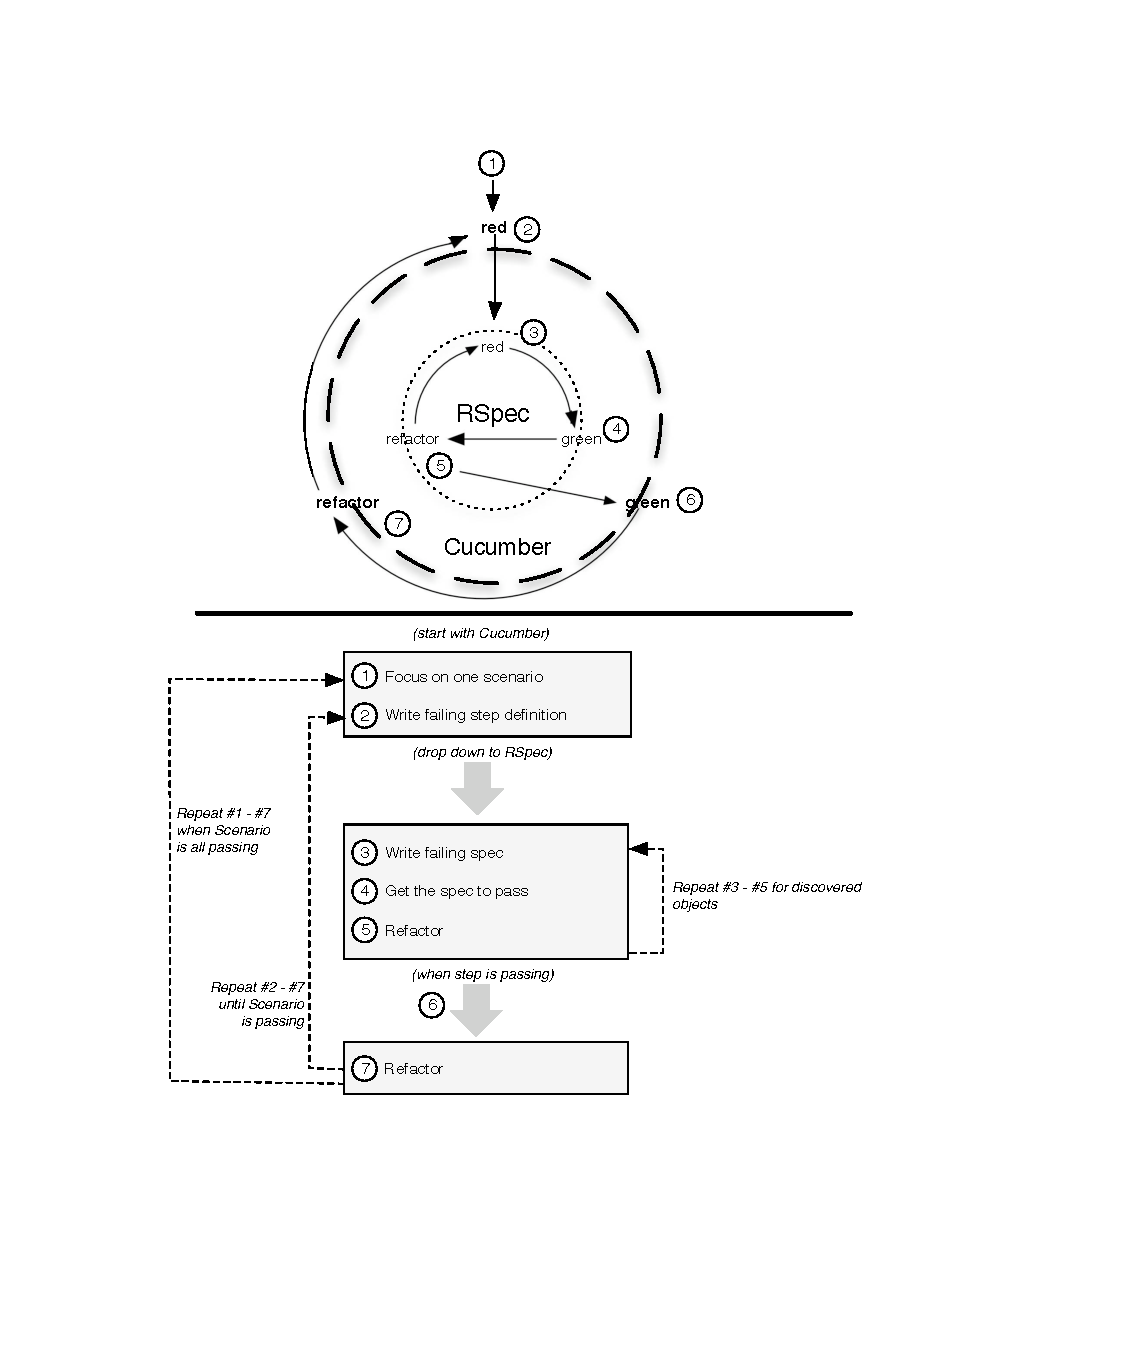
\includegraphics[width=0.9\textwidth]{diagrams/bdd_cycle.pdf}
  \caption{The BDD development cycle \cite{rspecbook}.}
  \label{bdd_cycle}
\end{figure}

%cycle, acceptance
At the beginning of the iteration an acceptance test is written and executing
it should reveal that the functionality is not yet implemented according to
it's requirements. Cucumber is a framework for writing acceptance tests in a
natural language as a set of steps in one or more scenarios.  An example
Cucumber acceptance test is included in Listing~\ref{cucumber_example}.

\bigskip
\begin{lstlisting}[label=cucumber_example,caption=Cucumber acceptance test example]
Feature: Logging
  As a webdeveloper
  I want to have logging of HTTP requests
  In order to debug errors or attacks on the webserver

  Scenario: Logging of HTTP requests
    Given the webserver is running
    When a user visits http://localhost/posts
    Then the log should contain "GET /posts"
    And the log should contain "SENT /posts SUCCESS"
\end{lstlisting}

The acceptance test in Listing~\ref{cucumber_example} covers the logging functionality of a webserver and tests it
by starting the webserver, making a request and then checking whether the log
contains the correct entry.  The first line names the feature covered by the
test. Lines 2 through 4 states the user of the feature, what it should do and
lastly why and what business value it creates. Line 6 states a specific
scenario, and often a feature has multiple scenarios and needs to test them
separately. Scenarios contains separate steps which defines either a
prerequisite (Given), an action (When) or a result (Then)\footnote{"And"
continues the previous step type}. The semantics of the steps are defined in a
set of step definitions written in Ruby.
Listing~\ref{step_definition_example} is a step definition of the step used on
line 9 in Listing~\ref{cucumber_example}.

\bigskip
\begin{lstlisting}[label=step_definition_example,caption=Cucumber step definition]
  Then /^the log should contain "([^"]*)"$/ do |entry|
    Server::log.should have(entry)
  end
\end{lstlisting}

The step definition checks whether the server log contains given entry using
RSpec. Steps are matched with regular expressions and \texttt{"([\^"]*)"}
matches the string "GET /posts" on line 9 in Listing~\ref{cucumber_example}.
Step definitions returns true if it passes and false if it didn't, and in the
case of a failure displays a detailed debug message.

%rspec -> red/green
RSpec is a BDD framework for Ruby used to write behaviour specifications
(specs). Specs are to BDD what unit tests are to TDD\@. Once the acceptance test is
written and run, steps will fail as they are not implemented (step 2 on
Figure~\ref{bdd_cycle}). Once implemented, steps might reveal application code
which is not yet available and therefore fail. In the example above, this error
could be caused by \texttt{Server} not having the method \texttt{log}. At this
point (point 3 on Figure~\ref{bdd_cycle}, an RSpec spec is needed to define the
behaviour of the \texttt{log} method. Listing~\ref{rspec_example} shows how such
a spec might look.

\bigskip
\begin{lstlisting}[label=rspec_example,caption=RSpec (spec) example]
describe Server do
  describe "#log" do
    it "should return an array" do
      Server.log << "Test string"
      Server.log.should.return(["Test string"])
    end
  end
end
\end{lstlisting}

Lines 1 and 2 in Listing~\ref{rspec_example} describes that we are specifying
the \texttt{log} method on the \texttt{Server} class. Line 3 describes the
intended behaviour of the \texttt{log} method; namely that it should return an
array. Then a test string is written to the log enabling the assertion that
calling the \texttt{log} method should contain that exact string. The next step
in the BDD cycle is now to get the spec to pass (go from red to green) with
the simplest solution possible. In case of the example, this would require
implementing the \texttt{log} method to return an array of log entries. Once
the spec passes, the code can be refactored if possible, and then the
developer moves on to the next failing step definition. This process is
continued until the acceptance test passes, meaning the feature is done and
behaves as intended.

\section{Webservers}
\label{webservers}
% \meta{Cover several webservers, each with their unique way of handling
%   concurrent requests.}

The goal of a webserver is to listen on a port for incoming requests, handle them
by either returning the contents of a file, run a program and return its
output, or return an error message if an error occurred. Since the Internet was
made public over 20 years ago, there have been countless webservers created, most
of which focus on handling websites written in a specific programming language
or framework. Multi-core processors have long been available in server
environments and hence, many webservers employ techniques to raise their
performance by handling HTTP requests in parallel.

This section looks at some of the available Ruby webservers and the
concurrency models they employ.

\subsection{Rack}
Rack is not an actual webserver, but an interface between webservers
supporting Ruby and Ruby web-frameworks. It is covered here as the Ruby
webservers covered next implement it. Rack decouples the link between the
webserver and web-application (written in one of the many Ruby web-frameworks) and
hereby makes it possible to change webserver without having to make any
changes to the web application. This is achieved by wrapping requests and
responses in a Ruby object. By implementing the Rack interface, a webserver
would immediately become compatible with more than 15 Ruby frameworks
\cite{rackspec}.

\subsection{Thin}
Thin is a webserver written in Ruby which include a HTTP parser written in C,
implements the Rack interface and uses EventMachine to handle requests in a
concurrent non-blocking manner \cite{thin}. EventMachine is a library which enables
event-driven (non-blocking) I/O by utilizing the reactor design pattern. The
reactor pattern works by having a dispatcher (reactor) passing on work to
various handlers, which then in turn fire an event when finished. This enables
Thin to focus on other requests instead of waiting on blocking actions such as
waiting for a file to be written to disk or fetching data from a remote API
\cite{reactor}.

Thin works by running the EventMachine event loop in a single thread, and
does therefore not employ any parallel processing, but does allow for
concurrency due to the asynchronous nature of the reactor pattern. Thin is
usually setup as a cluster of processes behind a proxy server or load
balancer.

\subsection{WEBrick}
WEBrick is a webserver which is included in the Ruby standard library. It is
written entirely in Ruby and employs concurrency by creating a separate thread
for each incoming request. WEBrick is mostly used as a development
server as it does not perform well under heavy loads due mainly to poor
performance of its HTTP parser \cite{webrick}.

\subsection{Unicorn}
Unicorn is a Ruby webserver which employs parallel processing by means of
forking separate worker processes \cite{unicorndocs}. It uses the same
C extension HTTP parser as Thin. By using processes, Unicorn allows for parallel
processing without the need to used a proxy server or load balancer as load
balancing is performed by the operating system.


\section{Concurrent Programming} % (fold)
\label{sec:concurrent}
Concurrency refers to code which is executed simultaneously on one or more
processors or cores in a single processor. Concurrent Programming refers to
programming language constructs which enables code to be executed concurrently.
Concurrent code executed on a single-core processor will look like it's executed
at the same time, but in reality the processor executes increments of each piece
of code by switching back and forth between them. The way a processor switches
between concurrent tasks is referred to as context-switching, and can easily bog
down a system as the context (program state and variables) needs to be loaded
for every context-switch.  Concurrent code executed on a multi-core processor
has the potential to execute code in parallel, e.g.\ at the same instance in
time. True concurrency can occur on a computer with either multiple processors
or one processor with multiple cores.

In most programming languages code is executed one statement at a time in a
sequential manner. Most programming languages does however include constructs
to allow for concurrent programming.  One of the most common constructs is
\textit{threads}. A thread is an abstraction for a piece of code which is
executed as a subroutine of the running program. This allows for executing
several threads concurrently or in parallel on multiple processors.  In
Section~\ref{sec:ruby}, the constructs available in Ruby are covered in more
detail.

Concurrency introduces several complications which must be taken into account,
mainly; race conditions and deadlocks. A race condition occurs when two or more
pieces of code tries to manipulate the same variable, and the outcome of the
program changes depending on the order of the manipulations. An example would be
if two threads, A and B, stored a counter in a global variable. Imagine thread A 
reads the value of the counter and then gets preempted and thread B changes
the counter and saves it. Then when thread A gets resumed it would have an
incorrect counter value, and changing the counter based on this would render
thread B's previous change. Race conditions can be fixed by synchronizing access
to shared resources such as variables. A common way too synchronize access to
shared resources is to add a mutual exclusion lock (mutex) around the code which
accesses the shared resource. A mutex could ensure that only one thread uses the
shared counter variable at a time. Deadlocks can occur when shared resources gets
locked by separate threads which then each waits for the other thread to
release the resource.

Race conditions occurring in a webserver could lead to erroneous data and
deadlocks could result in the server becoming unresponsive. Hence, they should
be avoided at all costs.

\section{Ruby} % (fold)
\label{sec:ruby}

%ruby in general
Ruby is an dynamic, reflective object-oriented general-purpose programming
language. It is dynamic in the sense that it is interpreted at runtime, and
reflective in the sense that it can modify and inspect program behavior during
runtime.  Ruby has a dynamic type system where the type of the object is
determined by what the object can do in terms of which methods are available
for the object. This type system is referred to as duck typing, i.e.\ if it
walks like a duck and talks like a duck, then the interpreter will treat it
like a duck.

The latest version of Ruby, version 1.9, holds several improvements over the
older but still maintained version 1.8. Besides small syntactic changes and
including a new VM, Ruby 1.9 introduced the concept of fibers. Ruby 1.9 also
includes RubyGems which enables easy packaging, installation and distribution
of Ruby software. RubyGems, mostly referred to as \textit{gems}, can be used
to modify or extend functionality within a Ruby application or to split out
reusable code for others to benefit from \cite{rubygems}. There are currently
over 27.000 gems available and this greatly reduces the need to "reinvent the
wheel", hence improving productivity. 

Ruby was chosen for this project because it is dynamic, expressive, productive
and terse, all adding to the speed and joyfulness of developing software.
Furthermore, Ruby has several constructs available for concurrent programming
which are covered below.

\subsection{Concurrency in Ruby}
Ruby comes with several constructs for concurrent programming; processes, threads
and fibers. The following describes the advantages and possible disadvantages
of each of these concepts.

\subsubsection{Processes}
A process is a running instance of a program, e.g.\ a running webserver or an
open text editor. Processes are handled by the operating system which
will utilize the available processors to run processes in parallel.
Hence, parallelism can be achieved by running multiple instances (processes) of
the same program.

Ruby includes a library for creating, killing and inspecting processes.
Creating a new process can be done by \textit{forking} a new process from the
current one. Forking starts a new Ruby VM with the executing program as a new
process. The forked and the original process does not have access to each
other memory, and thereby eliminates many of the problems regarding
race-conditions and deadlocks. The disadvantage of using multiple processes is
that, as they cannot easily share state, and they have to communicate through an explicit
protocol like inter-process communication \cite{ruby19}.

\subsubsection{Threads}
A thread is an encapsulation of a set of instructions which execution can
be managed. A thread can be seen as a lightweight process which has access to
the current programs memory. Threads are managed by a thread-scheduler which
decides when threads are run or preempted to enable other threads to
run. Using threads introduces complex issues as race-conditions can easily
occur due to all threads having access to the same memory.

An advantage of using threads is that they can easily share data, but that
is also one of it's disadvantages as it can easily become quite complex and
bugs concerning multi-threaded code can be very hard to discover
\cite{ruby19}.

\subsubsection{Fibers}
A fiber in Ruby is a coroutine mechanism which enables pausing and resuming
code blocks to achieve cooperative concurrency. A code block is a
piece of ruby code encapsulated in an object, and can be passed into
methods, saved in variables, and executed on demand. Fibers resembles threads in
that they can be controlled from outside, but whereas threads are managed by a
scheduler, fibers must be scheduled manually.

The advantages of fibers over threads are that they have a significantly lower
memory footprint and doesn't introduce the complexity of a scheduler \cite{rubyfiber}.

\subsection{Ruby Implementations}
Ruby code is run in a virtual machine (VM) of which there exists several
implementations. The official VM, for Ruby 1.9, is called YARV (Yet
Another Ruby VM). As there is no specification for Ruby, YARV serves as
the reference implementation for the Ruby language. The following describes
two widely used Ruby implementations, namely YARV and JRuby, and how they
differ in regards to concurrent programming.

\subsubsection{Yet Another Ruby VM}
YARV is developed and maintained as the official Ruby implementation and replaced
the old VM MRI (Matz\footnote{Yukihiro Matsumoto, a.k.a.\ Matz is the creator of 
the Ruby programming language} Ruby Interpreter) as of Ruby version 1.9. Given
YARV is the one driving the Ruby language implementation, it always has the
latest language features and updates, whereas other Ruby implementations tend
to be a bit behind. The latest stable version of YARV is 1.9.2, with 1.9.3
being just around the corner. YARV supports threads, fibers and processes, but
includes a Global Interpreter Lock (GIL) which limits the VM to only running
one thread at a time. The GIL is included to ensure non-threadsafe
C-extensions does not cause problems, and effectively bars YARV from
utilizing true parallelism from fibers and threads \cite{ruby19}.

\subsubsection{JRuby}
JRuby is a Ruby implementation that runs on any Java Virtual Machine (JVM)
and therefore enables using Java libraries from within Ruby. Java is a very
mature and large ecosystem with many useful libraries, language constructs and
concurrency models \cite{usejruby}.

JRuby does not include a GIL as YARV and therefore allows true
parallelism for threads, as opposed to only having one thread/fiber run
at a time. JRuby does however not support process forking as it is not
supported by the JVM\@ \cite{jruby}.

\section{Summary} % bsec

% \section{Literature Review} % (fold)
\label{sec:literature}

% section literature (end)

\newpage

\chapter{Analysis}
\label{an}
\meta{Should describe how and why I have decided upon the set of requirements.
  Given my choice of development method, there is not much design upfront,
        hence this section will only contain some initial thoughts on the
          structure of the software.}

In order to have a clear goal of what the software produced in this project
should do, a set of requirements are essential. 

As covered in Section\~ref{webservers}, the main purpose of a webserver is to
listen to HTTP requests, locate, and then return the resource or a response
according to the request. Hence, the webserver should be able to parse HTTP
requests in order to know how to respond. The parser should parse HTTP
requests according to the RFC 2616 specification.

In order to analyse and debug the webserver it should be able to log vital
messages to the console. This feature would greatly improve troubleshooting
and serve as a backlog of events in case of an error or an attack.

To increase the performance and throughput of the webserver it should handle
multiple requests at a time in a non-blocking manner. This would solve a slow
request blocking other requests from being processed.

The webserver should be able to serve static files like HTML, cascading
stylesheets, JavaScript and images in order to make webpages work as expected.
If no specific file is requested, then the webserver should return a HTML
formatted directory listing with links to the files in the given folder.

If a resources doesn't exist, or an error occurs during processing, the
webserver should return an error page with a short message on what went wrong.

The webserver should be able to webserver dynamic content by executing Ruby
scripts and returning their output. This enables client interaction instead of
simply being served static content.

In order to use the webserver with one of the many Ruby web-frameworks, it
should implement the Rack interface. This would instantly enable developers to
use the webserver with their web-applications.

\section{Requirements Specification}
The list below summarises the requirements for the webserver developed in this
project.

\begin{itemize}
  \item Parse HTTP/1.1 requests in accordance with RFC 2616.
  \item Logging of requests and responses.
  \item Handle concurrent requests in a non-blocking manner.
  \item Serve static files and directory listings.
  \item Return an error page if an error occurs.
  \item Serve dynamic content by executing Ruby scripts and returning the
  output.
  \item Implement the Rack interface
\end{itemize}

As this project was developed using BDD, the requirements specification was
translated into a set of acceptance tests to get concrete feedback on
completed requirements. The acceptance tests are included as
Appendix~\ref{acceptance_tests}.

\section{Project Planning}
Prior to starting development, the requirements were estimated and the
development split into several iterations, each driven by a requirement.
Figure~\ref{gantt} shows the initial planning of the development.

\begin{figure}[htb]
  \centering
  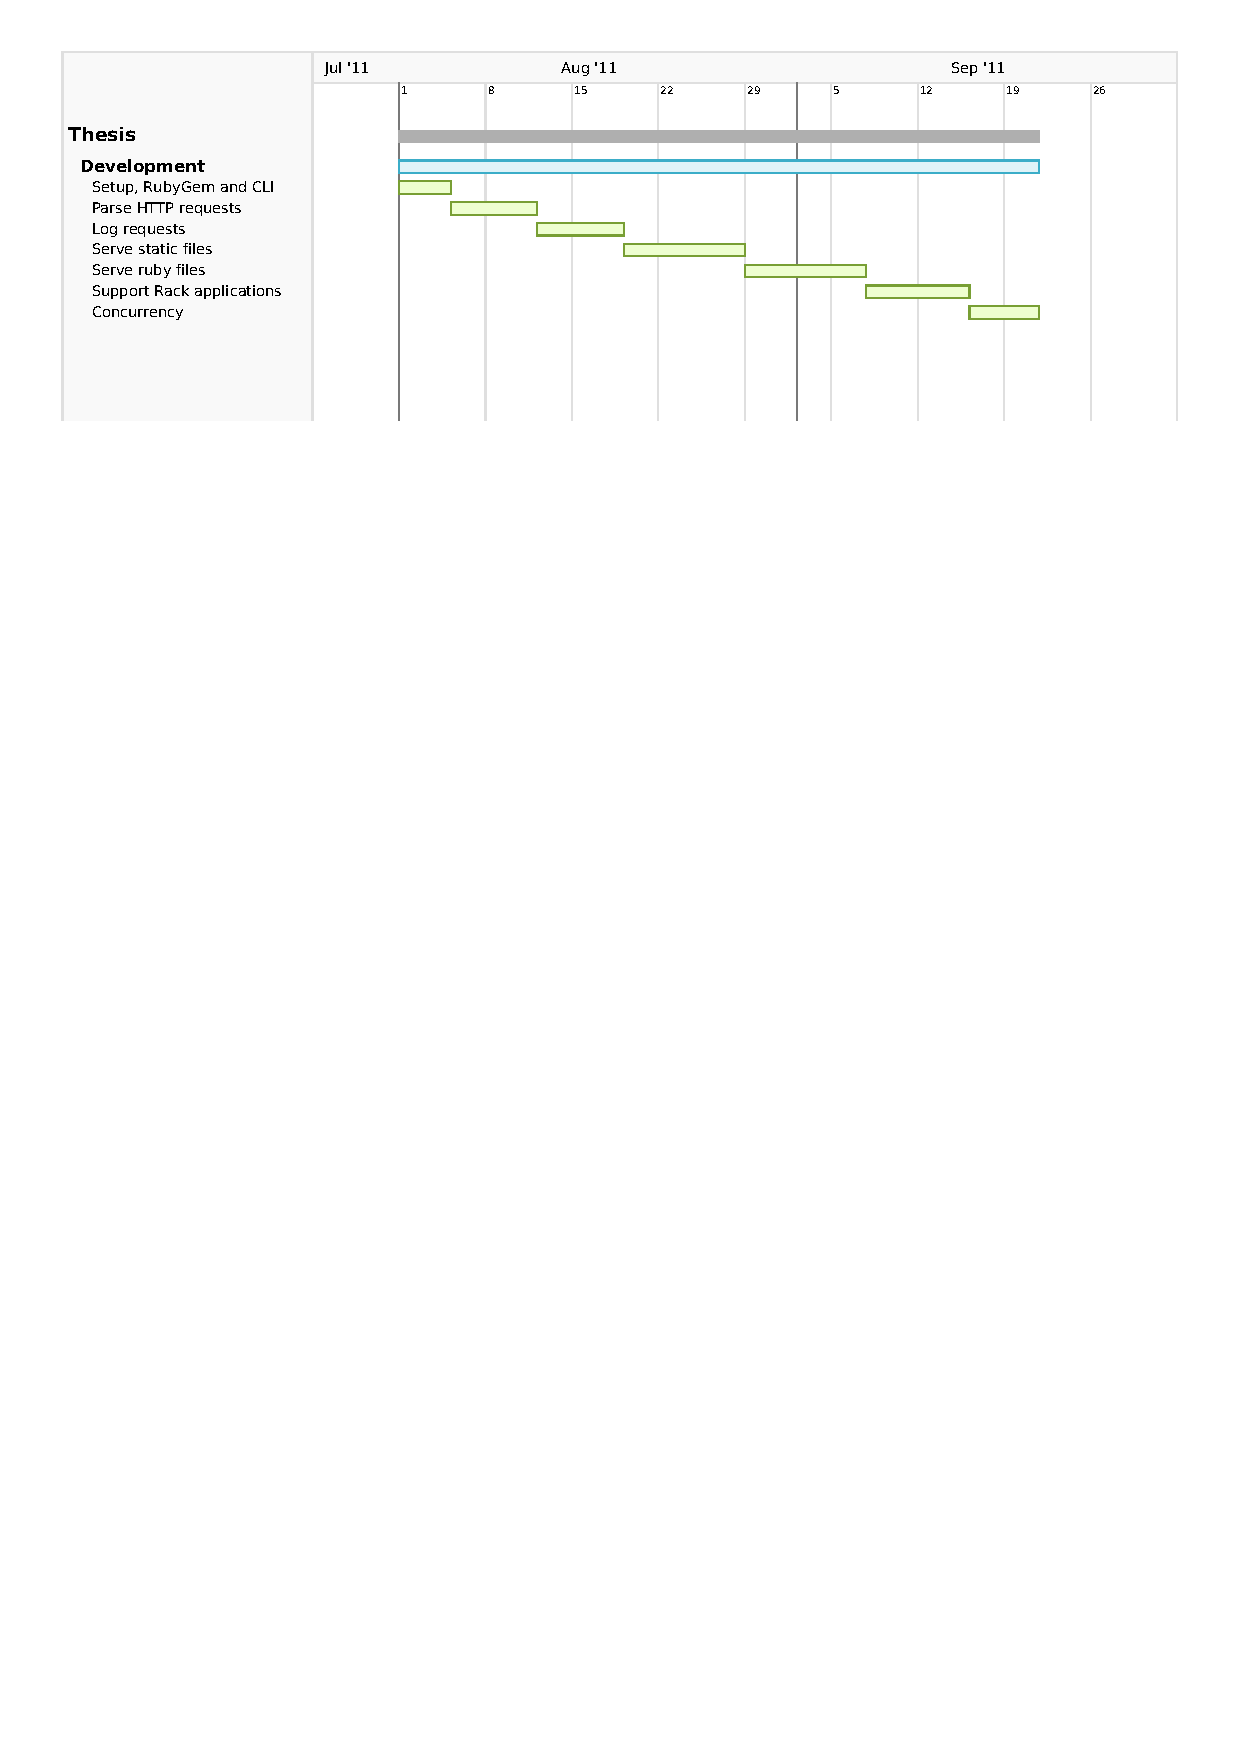
\includegraphics[width=1.0\textwidth]{img/gantt.pdf}
  \caption{Development Gantt Planning}
  \label{gantt}
\end{figure}

The development was planned to take place between August 1 and September 20.
The first three days were to be spent setting up the project, RubyGems
packaging and writing the command-line interface (CLI). Each requirement is
then implemented in turn, with varying time set aside, depending on the
complexity of the task.

As Behaviour-Driven Development was being used, no design was needed upfront,
and development could start head on. Design and architectural decisions were
to be made once the need arose, and tests were to be written prior to any
functionality.

\newpage

\chapter{Implementation}
\label{im}
% \meta{I choose to put implementation and testing together as that suits the
%   development method well. The chapter will contain interesting parts of the
%     implementation, problems which arose along the way and how I solved them.
% There is a section fore each of the requirements.}

Development of each requirement (see Section~\ref{req_spec}) was driven by
aiming to satisfy an acceptance test which stated the behavior of the feature.
The acceptance tests were written in a natural language using Cucumber, and
once the acceptance test passed the feature was considered done. All
requirements were satisfied, and this chapter covers some of the problems, and
their solutions, that occured during the eight weeks of development.

Initially, an overview of the webserver, it's parts and how it works is
described. Subsequently, selected interesting parts of the system is covered.

\section{System overview}
% \meta{The system as a whole. How it works with diagrams}

%intro
The user interface with Yarn through a Ruby script which accepts a
hostname and port number for to listen for incoming requests on, the number
of processes to fork and a Rack file. All parameters are optional, and default
values are used if none are given. By default the webserver will listen on
\texttt{127.0.0.1:3000}, with four worker processes serving static and dynamic
content. If a Rack file is given, then Yarn will serve requests by invoking
the Rack application. For debugging purposes, the user can supply a parameter
to include debug messages in the log. The following describes how Yarn handles
requests when serving static and dynamic files, and then how it serves Rack
applications.

When Yarn is started it will create a TCP server that listens for connections
on either the given or default port and hostname. If a Rack file is given,
then the application will be loaded. Then the process will fork into the given
number of workers and Yarn is ready to handle incoming requests. Each worker
contains a loop which, when registering an incoming connection, will call
either the \texttt{RequestHandler} or \texttt{RackHandler} depending on
whether a Rack application is loaded or not. Listing~\ref{worker_loop}
displays the loop run in each worker process.

\newpage
\begin{lstlisting}[label=worker_loop,caption=Worker loop
(Yarn/lib/yarn/server.rb:90)]
loop do
  @session = @socket.accept
  configure_socket
  handler.run @session
end
\end{lstlisting}

For each iteration the loop will wait at line 2 for an incoming connection,
and not busy-wait and run again. Once a connection is registered, the socket
is configured with some TCP optimizations and then the supplied to the
instantiated handler. The handler classes takes care of all the
rest and closes the connection when finished. If the user sends
the interrupt signal (usually by pressing Ctrl-c), Yarn will kill the worker
processes, close the TCP server and exit.

\section{Parser}
% \meta{describe how the parser works and the alternatives considered}

The HTTP request is received as a string of text, and in order to know the how
to respond, it needs to be checked for its validity. Furthermore, it should
be stored in a more convenient data format, to enable easier looking up
request information.

\subsection{HTTP Requests}
%RFC
The current version of the HTTP protocol, version 1.1, is well defined in a
specification called RFC 2616 \cite{rfc}. The specification clearly defines how
a HTTP request is formed and what it consists of. Listing~\ref{bnf} is an
excerpt from the specification and shows the overall structure of a HTTP
request.

\bigskip
\begin{lstlisting}[label=bnf,caption=HTTP request structure]
Request = Request-Line
          *(( general-header
           | request-header
           | entity-header ) CRLF)
          CRLF
          [ message-body ]
\end{lstlisting}

Listing~\ref{bnf} translates to; a \texttt{Request-Line}, followed by zero or
more headers, and after a \texttt{CRLF} an optional \texttt{message-body}.
Headers include information such as cookies present in the browser, browser
type, size of the \texttt{message-body}. \texttt{CRLF} is a newline (line
break), and is used to define the structure of the request, e.g.\ each
header is a separate line and an empty line separate the last header and the
\texttt{message-body}. The \texttt{Request-Line}, as shown in
Listing~\ref{reqline}, consists of a method, URI and HTTP version.

\bigskip
\begin{lstlisting}[label=reqline,caption=HTTP Request-Line]
Request-Line = Method SP Request-URI SP HTTP-Version CRLF
\end{lstlisting}

Listing~\ref{req_example} shows an example HTTP request.

\bigskip
\begin{lstlisting}[label=req_example,caption=Example HTTP request]
GET /path/file.html HTTP/1.1
User-Agent: Internet Explorer
Content-Length: 21

field=value&show=true
\end{lstlisting}

% different parsers
\subsection{Parsing Strategy}
The parser was written using a Ruby library named Parslet. Parslet works by
defining a set of rules and then applying them to check whether the input
satisfies the rules, and then extracts defined values. The rules consists of a
mix of regular expressions and boolean logic. Listing~\ref{parsersrc} shows the rule for the \texttt{Request-Line} as shown in Listing~\ref{reqline}.

\bigskip
\begin{lstlisting}[label=parsersrc,caption=Request-Line parser rule.
(Yarn/lib/yarn/parser.rb:61)]
rule(:request_line) do 
  method.as(:method) >> 
  space >> 
  request_uri.as(:uri) >> 
  space >> 
  http_version.as(:version) >> 
  crlf.maybe 
end
\end{lstlisting}

When a request is successfully parsed, a \texttt{Hash} containing the request
data is returned. E.g.\ running the parser on the example HTTP request from
Listing~\ref{req_example} will produce the following \texttt{Hash}:

\bigskip
\begin{lstlisting}[label=parser_out,caption=Example \texttt{Parser} output]
{ :method=>"GET"@0,
  :uri=>{:path=>"/path/file.html"@4},
  :version=>"HTTP/1.1"@20,
  :headers=>
    { "User-Agent"=>"Internet Explorer",
      "Content-Length"=>"21" },
  :body=>"field=value&show=true"@105 }
\end{lstlisting}

With the request formatted in a \texttt{Hash} it becomes very easy to
query information about it. The numbers in Listing~\ref{parser_out} preluded
by a @ denote the elements' start position in the request.

\section{Static and Dynamic Requests}
% \meta{Describe how static and dynamic files are served}
Serving static and dynamic content was developed as two separate features and
handler classes \texttt{StaticHandler} and \texttt{DynamicHandler}, but
later merged into what is now the \texttt{RequestHandler} class. From the
beginning it was clear that the handler classes would have much functionality
such as reading the request, invoking the parser and returning the response in
common, but also some distinct functionality. A way to vary an algorithm
whilst keeping much of the functionality the same is to use the Template
Method design pattern. The process of handling requests can be split up into
the following steps:

\begin{enumerate}
  \item Parse the request
  \item Prepare the response
  \item Return the response to the client
  \item Close the connection
\end{enumerate}

Given this process, the part that differs between handling static and dynamic
files is preparing the response. The Template Method makes provides a
convenient way to vary the implementation of how the response is prepared
\cite{design_patterns}.  Figure~\ref{template} shows how the relationship
between the handler classes.

\begin{figure}[htb]
  \centering
  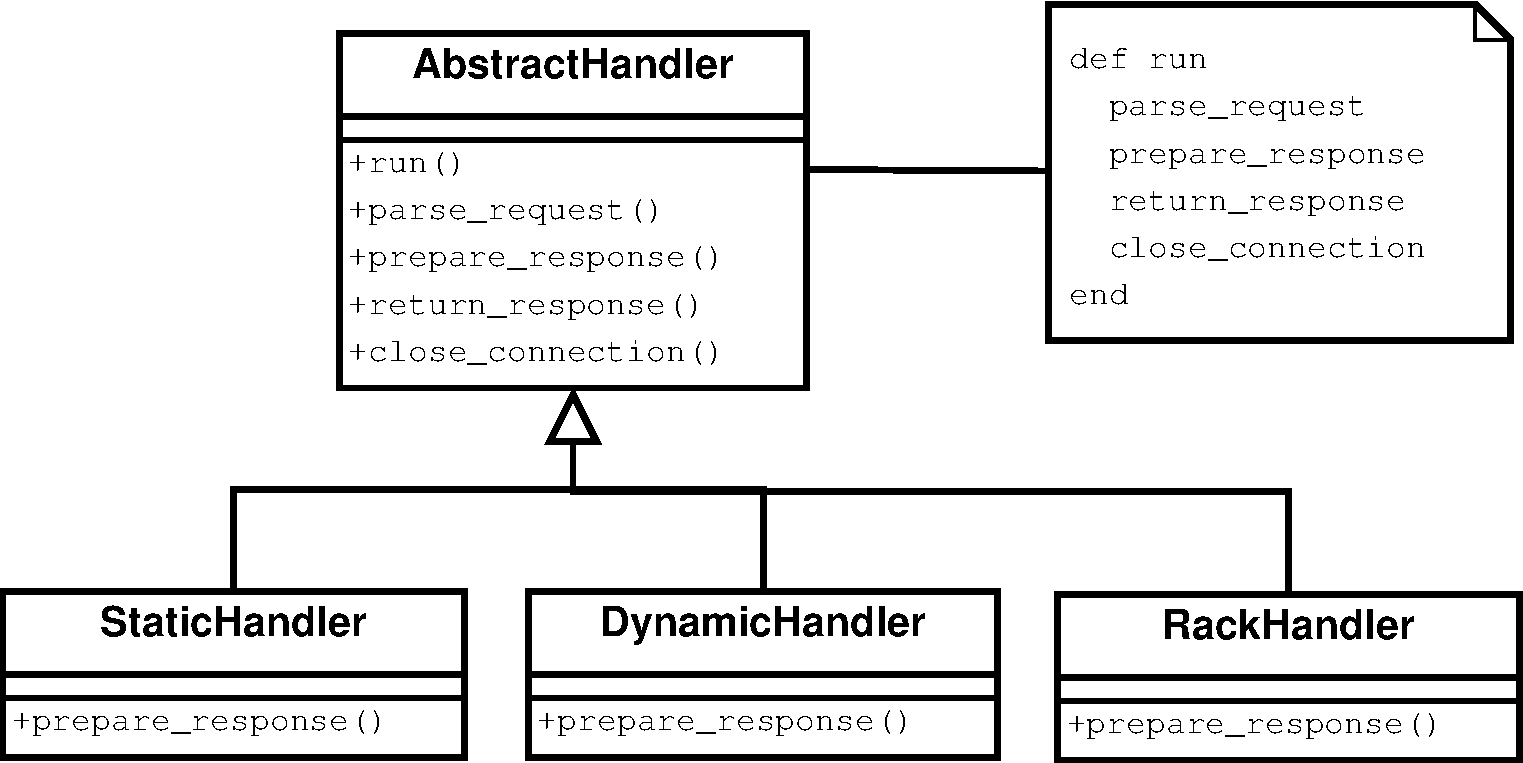
\includegraphics[width=0.7\textwidth]{diagrams/handlers.pdf}
  \caption{Initial handler implementation using the Template Method.}
  \label{template}
\end{figure}

Invoking run on each handler class would then follow the same process, but
each have their own implementation of \texttt{prepare\_response} method. Once
both handler classes were implemented it became clear that it would make more
sense to merge the two together to mirror how Yarn can be run to serve either
static and dynamic files or a Rack application. Figure~\ref{template2} shows
how the final handler classes were implemented (\texttt{RackHandler} is
covered in Section~\ref{rack}).

\begin{figure}[htb]
  \centering
  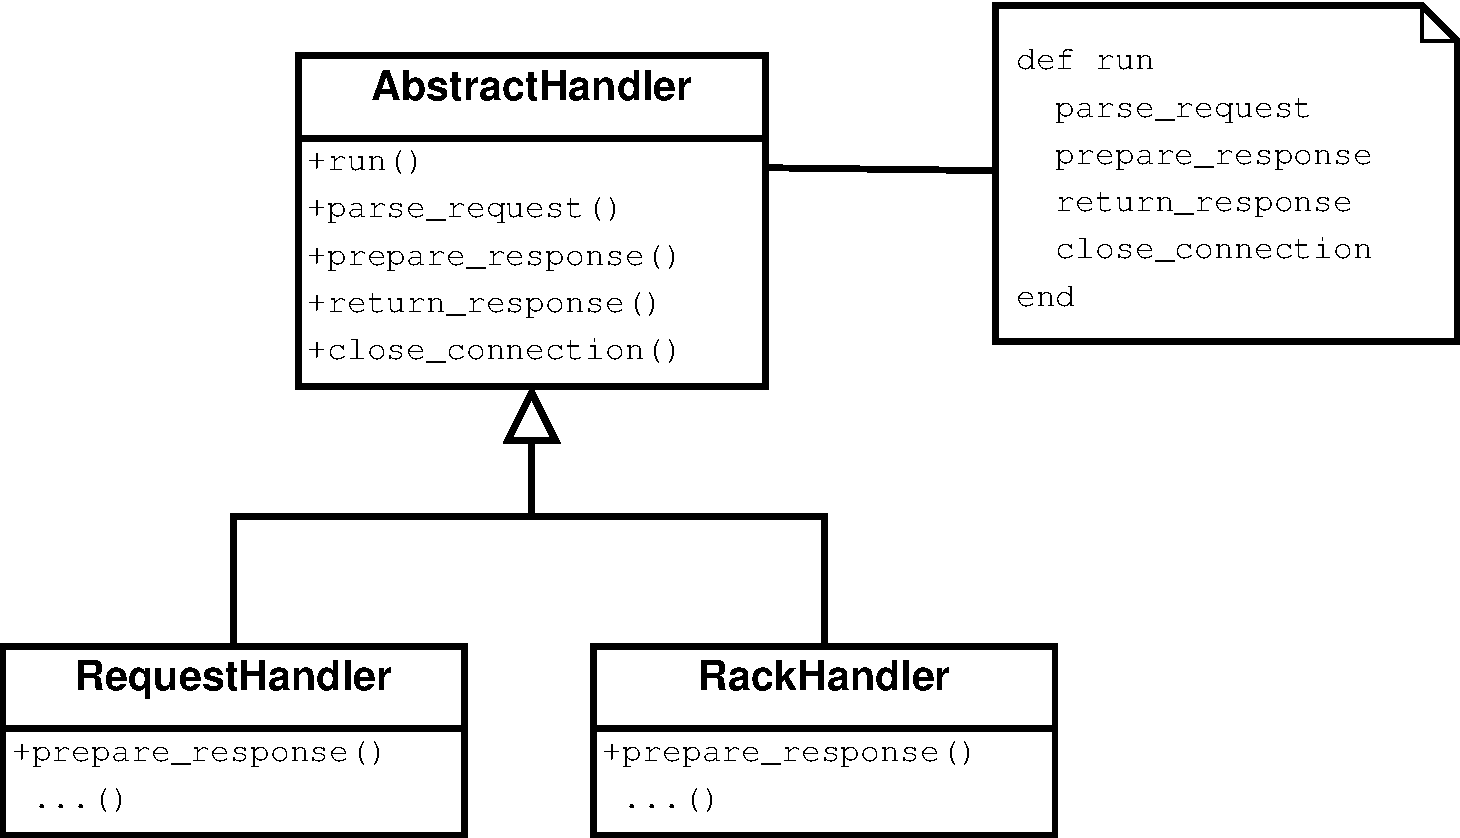
\includegraphics[width=0.7\textwidth]{diagrams/handlers2.pdf}
  \caption{Final handler implementation using the Template Method.}
  \label{template2}
\end{figure}

\subsection{RequestHandler}
\label{reqhandler}
The \texttt{RequestHandler} works by checking whether the requested path is a
file or a directory. Listing~\ref{reqhandle} show the logic
determining what is being served.

\begin{lstlisting}[label=reqhandle,caption=\texttt{RequestHandler} logic.
(lib/yarn/request\_handler.rb:8)]
begin
  if File.directory?(path)
    serve_directory(path)
  elsif File.exists?(path)
    path =~ /.*\.rb$/ ? serve_ruby_file(path) : serve_file(path)
  else
    serve_404_page
  end
rescue ProcessingError
  log "An error occured processing #{path}"
  serve_500_page
end
\end{lstlisting}

If the requested path is a directory, then a directory listing is served. In
case the requested file is ends with \texttt{.rb}, then it is executed and the
result is returned. In case the file does not exist or an error occurs
executing a Ruby file, then an error page is returned. Ruby files are executed
in the \texttt{execute\_script} method by evaluating the file using a new Ruby
VM and the result stored as the response body.



\section{Rack Applications}
\label{rack}
% \meta{describe how the Rack interface was implemented and what it required}
Implementing support for Rack applications consisted of two parts; loading the
Rack application and communicating requests and responses between the server
and the application.

Rack application are specified in a Ruby file which needs to be evaluated to
load the application. An example application is included which simply returns
a static array is included in Listing~\ref{rackex}.

\bigskip
\begin{lstlisting}[label=rackex,caption=Sample Rack application. (test\_objects/config.ru:4)]
run Proc.new { |env|
  [200, {'Content-Type' => "text/plain"}, ["Rack works"]]
}
\end{lstlisting}

When a Rack application file is supplied when running Yarn, the contents of
the file is read, passed into the \texttt{Rack::Builder} constructor which is
then evaluated. Listing~\ref{loadrack} contains the line where the Rack is
loaded.

\bigskip
\begin{lstlisting}[label=loadrack,caption=Loading a Rack application.
(lib/yarn/server.rb:31)]
  config_file = File.read(app_path)
  rack_application = eval("Rack::Builder.new { #{config_file} }")
\end{lstlisting}

Once loaded a Rack application is invoked with a \texttt{call} method which
returns an array containing the HTTP status code, HTTP headers and message
body. The The \texttt{call} method takes one parameter which is a
\texttt{Hash} of values the Rack application needs such as the path, hostname,
port, request body etc. \cite{rackspec}. 





\section{Concurrency}
Concurrency was developed lastly as to be able to properly test it with both
Rack applications and static and dynamic files. This section covers the stages
of development the concurrency feature went though, from using threads to
switching to processes.

\subsection{Initial Thread-per-request Implementation}
The initial implementation handled each incoming request in a new thread. This
however, quickly proved to introduce too much overhead in creating a new
threads. Furthermore, as the amount of threads hobbed up, memory use would
rise and eventually bog down the system. It became clear that another
solution was needed, and a system devised of a thread-pool and a job queue was
implemented. 

%thread pool
\subsection{Thread-pool and Job Queue Implementation}
The thread-pool was an array of threads, each running a handler which listened
for requests to be added to the job queue. Each incoming request would be added to
the job queue and then processed by one of the workers (handler in the
    thread-pool). The pros of this
solution was that, with a fixed number of threads, memory use was limited.
Furthermore, the job queue made sure that no requests were dropped if all
threads were busy serving other requests. 

Once implemented, several issues occurred which led to a rethink of the chosen
concurrency model. One problem was that requests would often hang indefinitely
and never return any content to the client. Exactly what caused this bug was
never discovered though many hours were spent trying the track it down. It was
suspected that the threads somehow created a deadlock which in turn would make
the client wait until the browser timed out.  Never discovering the cause of
the bug illustrates one of the key problems of threaded programming; bugs are
often very hard to replicate due to the complexity of the thread model and the
thread scheduler. 

Another problem with the thread-pool implementation was that it performed sub
par to the initial implementation of creating a new thread for each request.
This seemed to be caused by the way threads were scheduled, but again it
proved too difficult to pinpoint the exact cause of the poor performance.

Given the difficulty of a thread-based approach, it was decided to implement
the concurrency feature using processes instead.

%process model
\subsection{Process-based Implementation}
Implementing a process-based solution turned out to have many benefits, as it
both reduced the complexity of Yarn, but also greatly improved upon it's
performance.

The process-based solution was implemented by using \texttt{Process::fork}
from the Ruby standard library to fork new processes running the server. Each forked
process listens for incoming requests on the socket created in the master
process (the process which forked). Listing~\ref{processimpl} shows the logic for creating new processes.

\bigskip
\begin{lstlisting}[label=processimpl,caption=Process-based implementation
(Yarn/lib/yarn/server.rb:75)]
def init_workers
  @num_workers.times { @workers << fork_worker }
end

def fork_worker
  fork { worker }
end

def worker
  trap("INT") { exit }
  handler = get_handler
  loop do
    @session = @socket.accept
    configure_socket
    handler.run @session
  end
end
\end{lstlisting}

Once the \texttt{fork} method is called on line 6, a new process is started
with a separate Ruby VM and which continues on from that point. Meaning, each
process would invoke the \texttt{worker} method running the loop. On line 10, the
interrupt signal (INT) is trapped, such that when the user presses
\texttt{Ctrl-c}, all processes will exit and Yarn will stop. 

The process-based implementation improved the performance from $\sim$250
requests/second to $\sim$700 requests/second. The performance is covered in
more detail in Section~\ref{eval}. Another improvement of the process-based
concurrency model is that Yarn can now run on in parallel on YARV, wheres the
thread-based implementation would have to be run on JRuby to allow for
parallelism.


\section{Summary} % 
Throughout this chapter, parts of the implementation of Yarn have been covered.
It described how the parser, concurrency model and request handlers were
implemented and some of the troubles that arose during development. In the
next chapter, testing and how it is closely related to the implementation, is
covered.

\newpage

\chapter{Testing}
\label{te}
Throughout the development of Yarn, acceptance tests and specifications were
written prior to developing a feature. This provided a solid test coverage
which in turn allowed for some radical refactorings to improve the quality,
readability and performance of the system. By the end of development,
all 13 acceptance tests (Cucumber features) and 80 specifications (RSpec
specs) passed.  The final test coverage was 96.08\%, as depicted on
Figure~\ref{coverage}. 

\begin{figure}[htb]
  \centering
  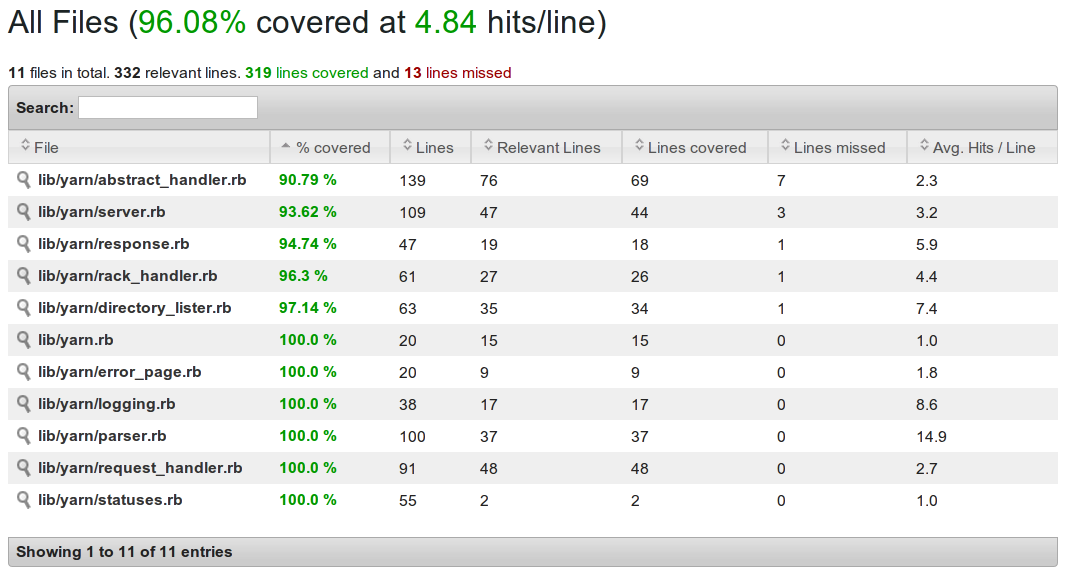
\includegraphics[width=0.9\textwidth]{img/coverage.png}
  \caption{Yarn test coverage screenshot.}
  \label{coverage}
\end{figure}

During the development, the test coverage was continuously monitored to ensure
all parts of the system were exercised in the test suite. The test coverage
analysis is available on the CD in the \texttt{coverage} folder. The following
looks at how testing for concurrency was performed, and how the HTTP parser
was developed with BDD.

\section{Testing for Concurrency}
Some features were harder to test than others, and testing for concurrency was
especially tricky. The solution was to invoke two requests to a Ruby file, 
which invoked the \texttt{sleep} method for a given amount of time before
returning the response. Firing a request which slept for a second would block
other requests from being served during that second. But if the server could
handle concurrent requests, a fast request fired after the slow request,
should be able to get its response prior to the slow request completing.
Listing~\ref{confea} shows the acceptance test for concurrent requests.

\bigskip
\begin{lstlisting}[label=confea,caption=Concurrency acceptance test
(Yarn/features/concurrency.feature:7)]
Scenario: Perform two requests in parallel
  Given the server is running
  Given a client "A"
  And a client "B"
  When client "A" makes a "1" second request
  And client "B" makes a "0.1" second request
  Then client "B" receives a response before client "A"
\end{lstlisting}

Having this acceptance test proved especially valuable during the
reimplementation of the concurrency feature from using threads to using
processes.

\section{Testing the HTTP Parser}
The development of the HTTP parser was initiated by writing an acceptance test
as shown in Listing~\ref{parsacc}.

\bigskip
\begin{lstlisting}[label=parsacc,caption=HTTP parser acceptance test
(Yarn/features/parser.feature:7).]
Scenario: Parse HTTP request
  Given a HTTP request "GET /index.html HTTP/1.1\r\nUser-Agent: cucumber\r\n"
  And a parser
  When I feed the request to the parser
  Then the result "method" should be "GET"
  And the result "uri" should include "path" with "/index.html"
  And the result "version" should be "HTTP/1.1"
  And the result "headers" should have "User-Agent" with "cucumber"
\end{lstlisting}

The acceptance test exercises the parser by supplying it with a HTTP request
string, and then expects the result to contain the values of the request.
Running the acceptance test revealed that the steps were not defined, and
implementing them was the next step. Listing~\ref{accstep} shows two of the step
definitions.

\newpage
\begin{lstlisting}[label=accstep,caption=Parser step definitions excerpt
(Yarn/features/step\_definitions/parser\_steps.rb:1).]
Given /^a parser$/ do
  @parser = Yarn::Parser.new
end

When /^I feed the request to the parser$/ do
  @result = @parser.run(@request)
end
\end{lstlisting}

With all the step definitions implemented, running the acceptance test again
revealed that the class \texttt{Yarn::Parser} did not exist. Creating the
class and running the test again revealed that the class did not have a method
named \texttt{run}. The development continued in this loop of first asserting
certain behaviour from the code, discovering it did not behave as asserted, and
then implementing the expected behaviour.

Each element which should be parsed was added incrementally by first writing a
RSpec specification, and then adding the behaviour to the \texttt{Parser}
class. For instance, the expected behaviour of being able to parse query
parameters was written in a specification (Listing~\ref{queryspec}).

\bigskip
\begin{lstlisting}[label=queryspec,caption=Parser query parameter support specification (Yarn/spec/yarn/parser\_spec.rb:54).]
it "parses query parameters in the URL" do
  result = Parser.new.run("GET /page?param1=1&param2=2 HTTP/1.1\n")
  result[:uri][:query].should == "param1=1&param2=2"
end
\end{lstlisting}

To begin with, the parser is executed with a HTTP request. Then the result
\texttt{Hash} is inspected to see whether the values match. Running the above
specification would output an error message as the parser could not yet
handle the query parameter. The behaviour, Listing~\ref{quepars} was then
added to the \texttt{Parser} class.

\bigskip
\begin{lstlisting}[label=quepars,caption=URL query parameter support (Yarn/lib/yarn/parser.rb:31).]
rule(:path) do 
  match['^\?'].repeat(1).as(:path) >> 
  str("?") >> 
  query.as(:query) | match['^\s'].repeat(1).as(:path)
end

rule(:query) do
  match['\S+'].repeat(1)
end
\end{lstlisting}

The behaviour added was lines 3,4 and lines 7 through 9. The path is checked
for the occurrence of a question mark, and if it is found the sequence of
characters until a whitespace character is parsed as the query string (line 8).

The implementation of all rules in the \texttt{Parser} class was developed
this way, totalling in 17 specs and one acceptance test for the
\texttt{Parser} class.


\section{Summary}
This chapter revealed how developing functionality through first describing
the expected behaviour in a test, worked out well and always made it clear
what the next step to completing a feature would be. It was also covered how
using a tool to monitor test coverage, ensured that all execution paths were
tested and thereby improved the value of the test suite.
In the next chapter the final version of Yarn is demonstrated and benchmarked.


\chapter{Demonstration and Benchmark}
\label{de}
\section{Demonstration}
\meta{Briefly show screenshots and how the server works and is distributed}


\section{Evaluation}
\label{eval}
To evaluate Yarn, it's performance will be analyzed first by itself, then it
is compared to the other Ruby webservers covered in Section~\ref{webservers}.
The measure of performance is how many requests the webserver can handle per
second. The tests were run on a Linux machine with four cores and 8GB RAM.

\subsection{Yarn Performance}
To get an idea of the performance of Yarn, it was measured how many requests
per second (req/sec) it could handle at different counts of worker processes.
Figure~\ref{optwork} plots Yarn performance.

\begin{figure}[htb]
  \centering
  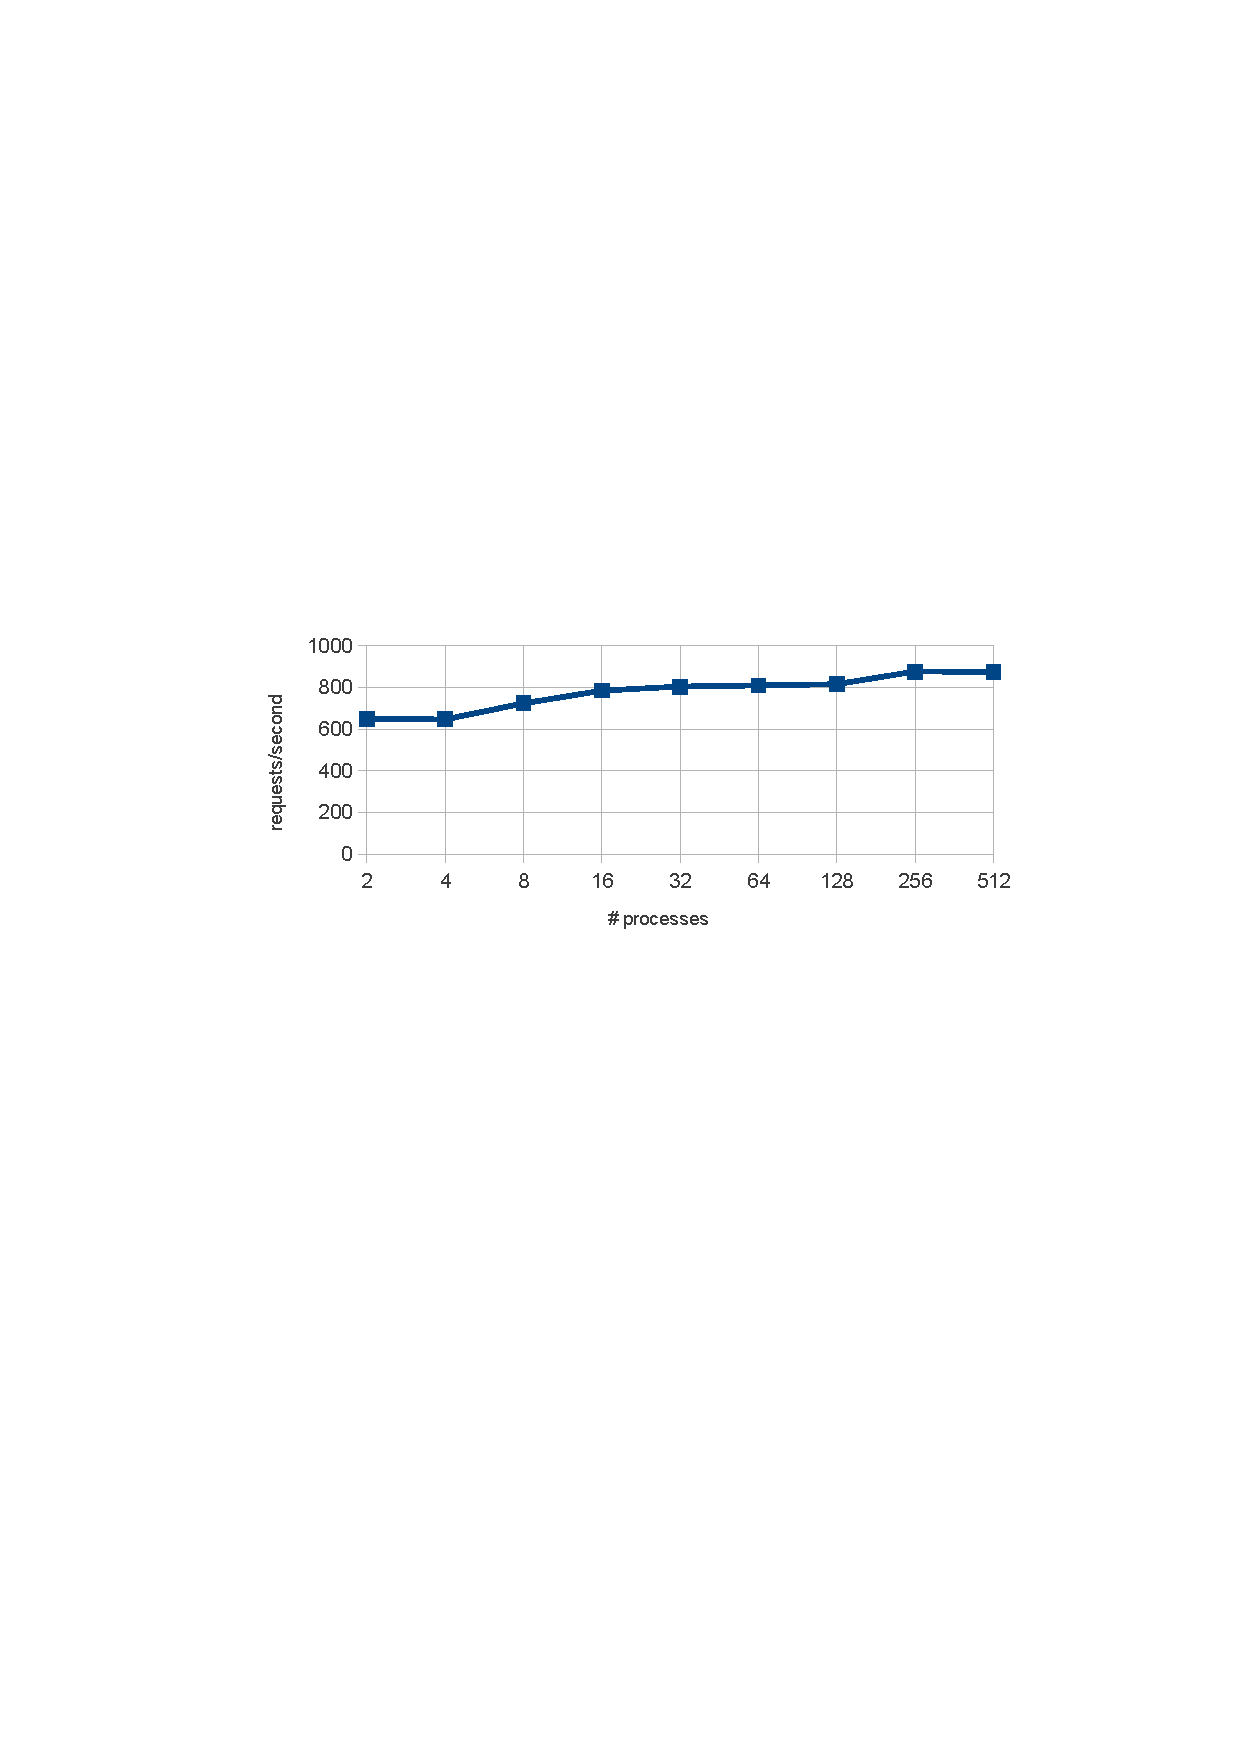
\includegraphics[width=1.0\textwidth]{results/optimal_workers_crop.pdf}
  \caption{Yarn req/sec}
  \label{optwork}
\end{figure}

Test runs above 512 processes bogged the computer down and were not included.
The best result was achieved with 256 worker processes with 875
req/sec, and on average Yarn performed 775 req/sec. The test consisted of
making 1000 requests, 20 at a time, to Yarn serving a simple Rack application.

\subsection{Yarn Vs. Other Ruby Webservers}


\newpage

\chapter{Critical Evaluation}
\label{re}
This chapters looks critically at the final product and reflects upon the
project process using Behaviour-Driven Development.

\section{Product Evaluation}
The final version of Yarn (0.1.0) includes all features from the requirement
specification, and all acceptance tests and specifications passes. 

Yarn is stable with \textgreater 10 worker processes and at low request
volumes. However, when the requests to worker process ratio becomes too high,
some TCP connections are dropped and no content is delivered to the client.
It was not possible to fix this bug as no more time was left for
development.

The performance of Yarn is quite satisfying for CPU intensive applications,
but for static content it performs subpar to other Ruby webservers.
\fixme{blame parser?}

\section{Process Reflection}
Developing software tests first proved to be difficult at times when it was
hard to figure out how a piece of code would even work. Having done mostly
non-test-first development prior to this project, it required a continous
concious effort to stick to writing tests before implementing features. Late
in the development phase, it became a more natural effort to drive the
implementation thorugh testing, and the advantages of the workflow were proved
a great asset. Having the tests provided the courage which was sometimes
needed prior to a large rewrite of refactoring of a feature, as it was always
easy to see whether the changes had broken the system. Furthermore, by writing
the tests first, it was always clear what the next step was as running the
test would reveal exactly what was missing in the implementation.

Given there was no design phase prior to starting the development, the design
desicions were made continously throughout the development. This resulted in
some desicions made early on which later proved to be less fortunate. But due
to the agile nature of BDD, and the confidence achieved by having a big test
suite, drastic design changes late in the process were possible. Had the
system been thoroughly designed upfront, such drastic changes might have been
fatal to the success of the project.

\newpage

\chapter{Conclusion}
\label{co}
% \meta{The conclusion should summarise the work and the final product.}
% What the thesis sai
\fixme{still a draft}

BDD works well, but can be hard with new technology. As a design flaws are
detected which might have been prevented with a more thorough design upfront.

For most applications, processor power is not an issue. Whats more important
are disk and network IO.


\section{Future Work}
% \meta{Covers which what could be improved if more time was available}
Given more time for development, there are a number of imminent features and
a bug which should be added or fixed before Yarn will be stable enough to be
used in a production environment.

The bug regarding dropped TCP connections should be fixed, possibly by
enqueuing incomming requests to make sure requests are being properly served
even at hight volumes. Implementing a request queue with the current process
concurrency model will require some form of inter-process communication
protocol.

%Support keep-alive connections to save TCP overhead.
Yarn currently does not support persistent TCP connections, and for each
request, a new TCP connection is used. This creates an overhead which could be
spared by allowing clients to reuse existing connections.

%opensource.
The source-code for Yarn is open-source and publicly available on Github which
is a web-based collaborative Git hosting site. This enables anyone to suggest
or add improvements and features to the project for the good of all Yarn
users. Given time to mature and possible interest from the Ruby community,
Yarn might evolve to be a prominent Ruby webserver.

\newpage

\label{theend}

% Bibliography 
\bibliographystyle{plain}
\bibliography{references/Thesis,references/manual}
% \nocite{*}
\label{bib}

% Appendix
% \appendix
% \appendixpage
% \chapter{Acceptance Tests} % (fold)
\label{acceptance_tests}

\begin{lstlisting}[label=act0,caption=acceptance test.]
Feature: Server control

  As a developer
  I want to be able to command the server
  So that I can control the server

  Scenario: Start server
    When I start the server on port 3000
    Then I should see "Server started on port 3000"

  Scenario: Stop server
    Given the server is running
    When I stop the server
    Then I should see "Server stopped"
\end{lstlisting}



\label{pagecount}

\newpage
\listoffixmes
\addcontentsline{toc}{chapter}{Todo}

\end{document}
